\section{APPENDIX}


\subsection*{Implementation of Hit-and-Run}
The polytope $P$ is defined by the mechanics of the limb and the constraints of the task as
\[\textbf{f} = A\textbf{a}, \textbf{a} \in [0,1]^n,\]
and to find a starting point $\textbf{p}$ we  need only to find one feasible activation vector in the space.
For the Hit-and-Run algorithm to mix faster we do not want the starting point to be close to a vertex of the $n$-cube \cite{Lovasz}. Intuitively, this is because a random direction from that point will be able to `travel far' from the corners in $P$.
We use the following standard trick with slack variables $\epsilon_i$, which in practice often provides a good starting point for sampling algorithms. In essence, we use the slack variables to shrink the extreme values of the variables to find a solution that is in the core of the $n$-cube. [state the value of $\epsilon$]

\begin{equation}\label{eq:LP_r}
\begin{array}{lrcl}
\mbox{maximize} & \sum_{i=1}^n \epsilon_i \\ 
\mbox{subject to} & \textbf{f} &=& A\textbf{a}\\
  & a_i &\in& [\epsilon_i, 1- \epsilon_i], \hspace{5mm} \forall i \in \{1,\dots,n\}  \\
  & \epsilon_i &\geq& 0, \hspace{5mm} \forall i \in \{1,\dots,n\}.  
\end{array}
\end{equation}
Thus running a linear program with these reduced ranges of the variables will produce a starting point that is far from the extremes of the actual $n$-cube.

The rest of the implementation of the Hit-and-Run algorithm is straight forward except for the choice of the random direction. How do we sample u.a.r.\ from all directions in $P$? 
Recall that all points in $P$ are by definition valid solutions to a given task. Therefore you can think of  $P$ as the null space of the task. Thus moving from  point $\textbf{p} \in P$ by the displacement vector  $\textbf{q} \in P$ takes you to another valid point $\textbf{p'}=\textbf{p}  + \textbf{q}$ that in fact produces the \emph{same output}
Thus, by the definition of $P$ as the feasible activation set, the direction $\textbf{q}$ must satisfy $\textbf{f} = A(\textbf{p}+\textbf{q})$. Since $\textbf{p} \in P$, we know that $\textbf{f} = A\textbf{p}$ and therefore 
\[\textbf{f} = A(\textbf{p} + \textbf{q}) = \textbf{f} + A\textbf{q} \Rightarrow A\textbf{q} = 0. \]
This essentially says that the direction $\textbf{q} $ must be in the null space of the task, which is defined as  $A\textbf{x} = A(\textbf{x} + \delta\textbf{x})$ if $\delta\textbf{x} \in N(A)$. 

Hence we need to choose directions uniformly at random across the vector space 
\[V = \{\textbf{q} \in \mathbb{R}^n | A\textbf{q} = 0\}.\]

As shown by Marsaglia this can be done as follows \cite{Marsaglia}.
\begin{enumerate}
\item
Find an orthonormal basis $b_1, \dots, b_r \in \mathbb{R}^{n}$ of \{$\textbf{q} \in \mathbb{R}^n | A\textbf{q} = 0$\}.
\item
Choose $(\lambda_1, \dots, \lambda_r) \in \mathcal{N}(0,1)^r$ (from the zero-mean unit-variance Gaussian distribution).
\item
$\sum_{i=1}^r \lambda_i b_i$ is a u.a.r.\ direction.
\end{enumerate}

A basis of a vector space $V$ is a minimal set of vectors that generate $V$, and it is orthonormal if the vectors are pairwise orthogonal (perpendicular) and have unit length. Using basic linear algebra one can find a basis for $\{q \in \mathbb{R}^n | A\textbf{q} = 0\}$ and orthogonalize with the well known Gram-Schmidt method (for details see e.g.\ \cite{Robertson}). Note that in order to get the desired u.a.r.\ sample the basis needs to be orthonormal. [let's discuss this: The limb model is defined such that the rows of $A$ are linearly independent and hence $r=n-m$.]

\subsection*{Mixing Time}
\label{sec_lengthrun}
From a given starting point, how many iterations of the Hit-and-Run method are necessary to reach a u.a.r.\ point.
For convex polytopes in $n$ dimensions up to $40$, experimental results suggest that $\mathcal{O}(n)$ steps of the Hit-and-Run algorithm are sufficient.
In particular, the paper \cite{emiris2013efficient} by Emiris and Fisikopoulos suggests that selecting every $10(n + 1)$ points is sufficient to get a uniform distribution \cite{emiris2013efficient}, while in Ge et al.'s paper every single point of the Hit-and-Run algorithm is used in the sample \cite{Ge}.


The Hit-and-Run algorithm was specifically developed to address $\#P$-hard problems such as approximating the volume of high-dimensional polytopes\cite{Dyer}. The Hit-and-Run algorithms can converge to the uniform sampling across any convex body \cite{smith1984efficient} after $\mathcal{O}^*(n^2R^2/r^2)$ steps ($r$ and $R$ are the radii of the inscribed and circumscribed ball of the polytope as mentioned in the Introduction) \cite{Dyer, Lovasz}.  Experimental results  suggest that a number of points linear with respect to $N$  suffices for convex polytopes embedded in dimensions up to 40.  Emiris and Fisikopoulos \cite{emiris2013efficient} suggest that  $(10 + \frac{10}{N})~N$ iterations suffice to uniformly sample a convex polytope.





\subsection{Finger model data}
$F_0 = (123.0, 219.0, 23.52, 91.74,	21.6, 124.8, 129.6)$\\
$
JR = 
\begin{pmatrix}
-0.08941 & -0.0447 & -0.009249 & 0.03669 & 0.1421 & 0.2087 & -0.2138 \\
-0.04689 & -0.1496 & 0.052 &0.052 & 0.0248 & 0.0 & 0.0248 \\ 
0.06472 & 0.001953 & -0.1518 &-0.1518 & 0.2919 & 0.0568 & 0.2067 \\
0.003081 & -0.002352 & -0.0001649 & -0.0001649 & -0.0004483 & 0.0001578 & -0.000685
\end{pmatrix}$

Distal force is $task_z = (0.0,0.0,1.0,0.0)$

\begin{figure}[h]
\centering
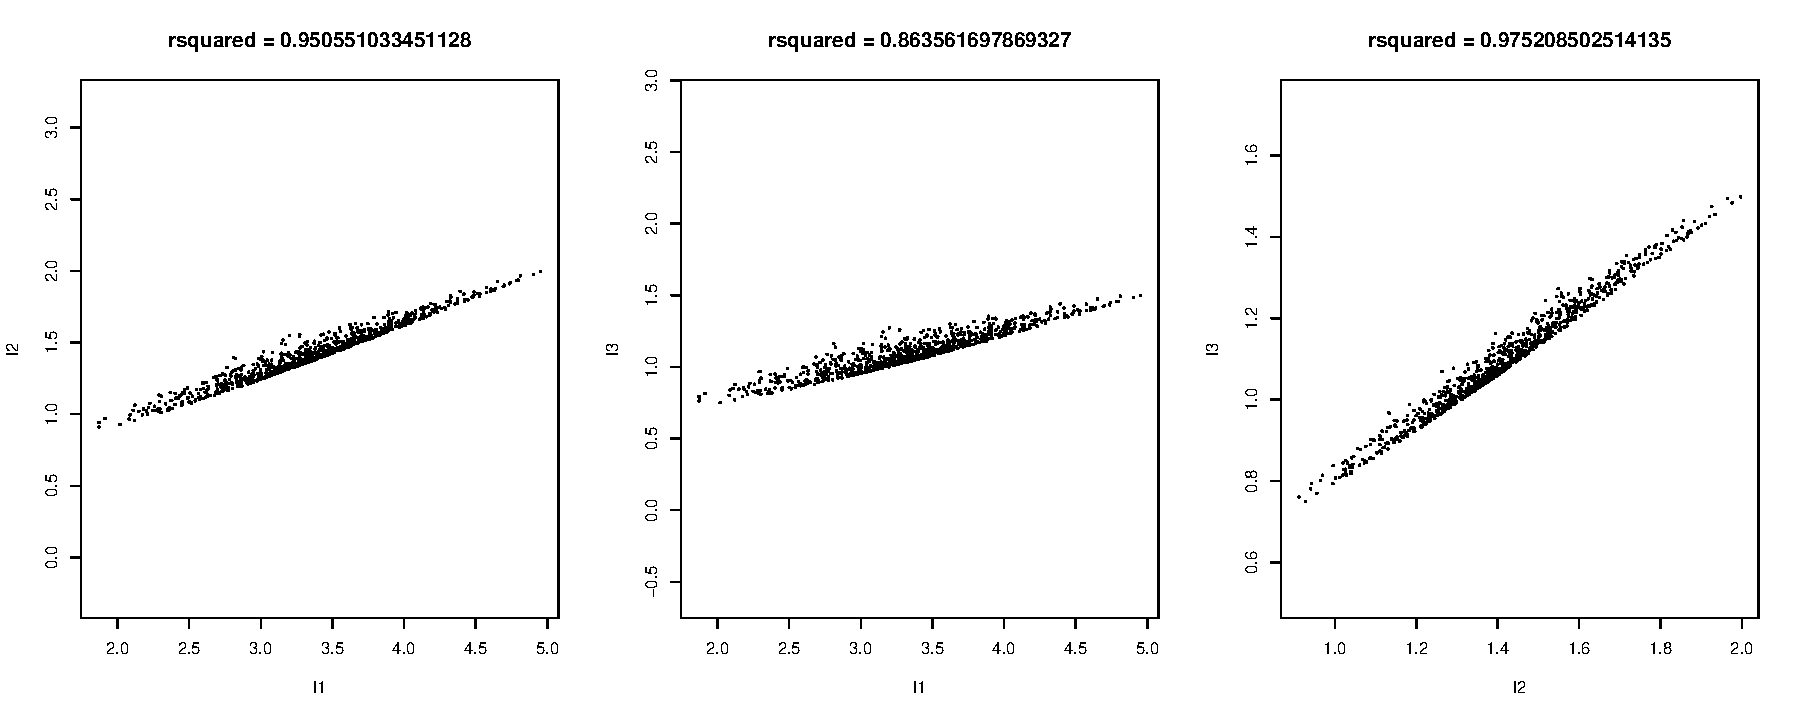
\includegraphics[width=\textwidth,page=1]{figs/cost_function_scatterplots.pdf}
\caption{Non weighted cost functions}
\label{fig:unweighted_cost_functions}
\end{figure}

\begin{figure}[h]
\centering
\includegraphics[width=\textwidth,page=2]{figs/cost_function_scatterplots.pdf}
\caption{Weighted cost functions}
\label{fig:weighted_cost_functions}
\end{figure}
The result of these computations (evaluated in R) shows the cumulative percentage of points up to each of those points.
\begin{verbatim}
# fixed_db database where each row is a point, each column is a muscle, and one column is the alpha level
library(stats)
eip_solutions <- fixed_db[fixed_db['alpha']==0.9,][,3]
activations_of_interest <- c(0.49,0.51)
ecdf(eip_solutions, activations_of_interest)
\end{verbatim}

We developed and tested our code in  Ubuntu 14.04, Windows 8.1, and OSX Yosemite 10.10.3; implemented Hit-and-Run with Scala 2.11.6\footnote{http://www.scala-lang.org/}, developed our histograms and descriptive statistics with R 3.1.3 \cite{rCoreCitation}, and designed our parallel coordinate visualization with multiple open-source JavaScript projects \footnote{http://syntagmatic.github.io/parallel-coordinates/}\footnote{http://d3js.org/}.
All code and documentation used to develop this publication is readily available on a Github repository \footnote{https://github.com/bcohn12/space}
